\documentclass[12pt,a4paper]{article}
\usepackage{amsmath}
\usepackage{amsfonts}
\usepackage{amssymb}
\usepackage{graphicx}
\usepackage{secdot}
\usepackage[left=2cm,right=2cm,top=2cm,bottom=2cm]{geometry}

\title{Experiment - 2\\Flow through a pipe of sudden expansion}
\author{Arka Pramanick, AE21B007\\ Department of Aerospace Engineering\\ IIT Madras\\[3ex] Instructor:\\ \large Professor Dr. R. Sriram}

\date{07 February, 2023}


\begin{document}
\maketitle

\hline

\section{Aim :}
To determine Head loss due to flow through a pipe of sudden expansion.   
\section{Apparatus :}
Required apparatus for performing this experiment are:
\begin{itemize}
    \item A digital manometer (for measurement of pressure)
    \item Pipe  with 3 different diameters and of sudden expansion
    \item A fan
\end{itemize}
\section{Theory :}
\begin{figure}[!ht]
	\begin{center}
		\framebox{
			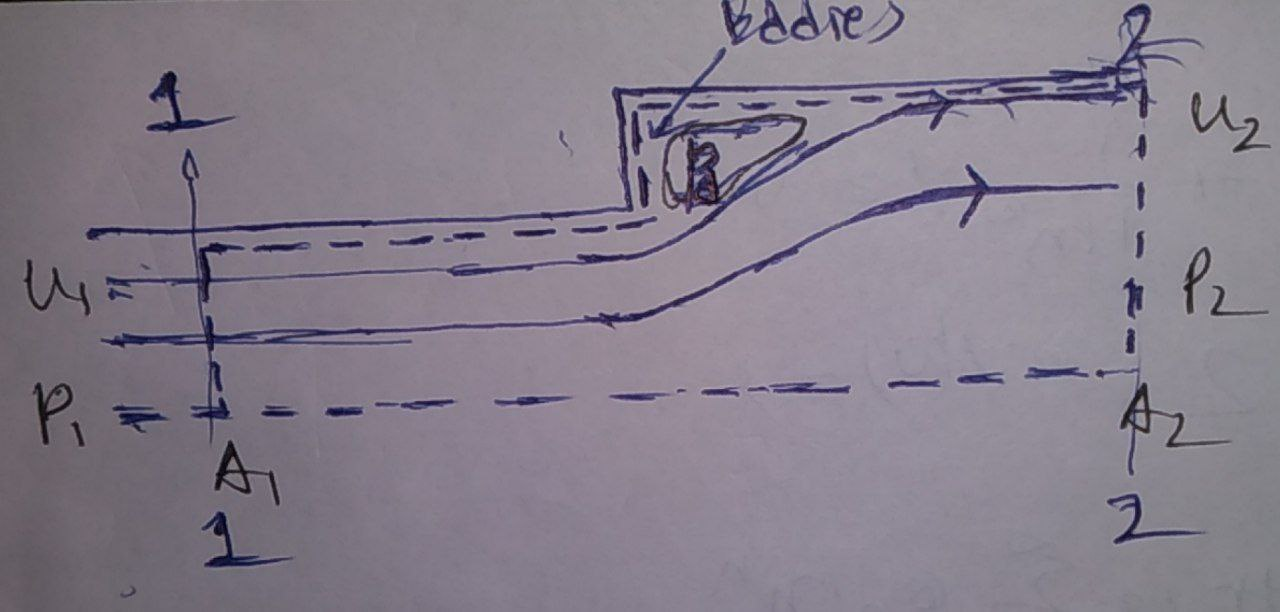
\includegraphics[scale=0.4]{photo_6273810045716247643_y.jpg}
		}
	\end{center}
	\caption{Headloss due to sudden expansion for flow through a pipe}
\end{figure}
A horizontal pipe(as shown in figure) of area $A_1$ is suddenly enlarged to the area $A_2$

Section 1-1 : Section before expansion.
Section 2-2 : Section after expansion.
$P_1,A_1,u_1$ is the pressure,area and velocity at section 1-1.\\
$P_1,A_1,u_1$ is the pressure,area and velocity at section 2-2.\\
$P_d$ : Pressure of the fluid eddies on the area $(A_2-A_1)$.\\
Due to sudden enlargement in the diameter of pipe eddies are formed at the corners of the enlarged pipe which results in head loss across the fitting.

From equation of mass flow rate(Q) :
\begin{equation}
    A_1 u_1 = A_2 u_2 = Q\\
\end{equation}
\begin{equation}
    A_1/A_2 = \alpha = u_2 /u_1
\end{equation}
Applying Bernoulli's equation between section 1-1 and 2-2 :
\begin{equation}
    P_1 + \frac{\rho_1 u_1^{2}}{2} = P_2 + \frac{\rho_2 u_2^{2}}{2} + H_l 
\end{equation}
Momentum Equation.:
\begin{equation}
    \rho A_2 u_2^{2}-\rho A_1 u_1^{2} = \rho Q (u_2 - u_1) = P_1 A_1 + P_d(A_2-A_1)-P_2A_2
\end{equation}
Generally it is observed that : $P_d \approx P_1$\\
So the momentum equation becomes :
\begin{equation}
    \rho A_2 u_2(u_2 - u_1) = A_2 (P_1-P_2)
\end{equation}
\begin{equation}
    P_1-P_2 = \rho u_2(u_2-u_1)
\end{equation}
Using eqn(6) and eqn(2) in eqn(3) we get,
\begin{equation}
    H_l = \frac{\rho u_1^{2}(1-\alpha)^{2}}{2}
\end{equation}


\section{Procedure :}
\begin{enumerate}
    \item First fix the desired ports across the length of pipe of sudden expansion in the manometer.
    \item Gradually increase the speed of wind flowing inside after starting the machine.
    \item Take readings at that particular ports.
\end{enumerate}






\section{Observation :}

\subsection{Gauge pressure variation across the length of the pipe :}
 
\begin{table}[ht]
 \centering
 \caption{\textbf{Variation of Gauge Pressure across length of pipe starting from nozzle}}
\vspace{2mm}
\begin{tabular}{ |c|c| } 
 \hline
 \textbf{Distance from starting of nozzle(in mm)} & \textbf{Gauge Pressure (in KPa)}  \\ 
 \hline
  0 & - 0.4 \\ 
 \hline
  9 & -0.9 \\ 
 \hline
 36 & -9.9 \\ 
 \hline
 84 & -11.1 \\
  \hline
 94 & -11.3 \\ 
 \hline 
 150 & -9.9 \\
 \hline
\end{tabular}
\end{table}
\begin{figure}[!ht]
	\begin{center}
		\framebox{
			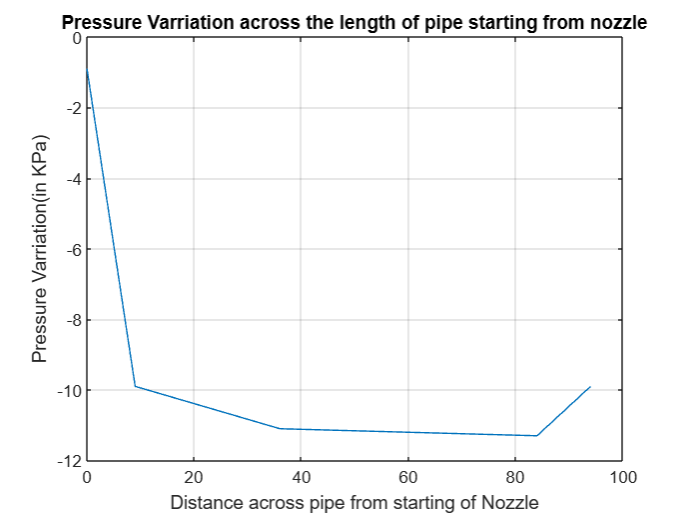
\includegraphics[scale=0.6]{ls2 graph1.png}
        }
	\end{center}
	\caption{Pressure Variation vs Distance across pipe starting from Nozzle }
\end{figure}
\newpage
\subsection{Pressure variation across length of for different set of data and corresponding velocity}
\begin{table}[ht]
\centering
\caption{\textbf{Pressure variation at different distance of Pipe and corresponding flow velocity}}
\vspace{2mm}
\begin{tabular}{ |c|c|c|c|c|c|c|c| } 
 \hline
 \textbf{S.No.} & $P_1$ & $P_2$ & $P_3$ & $P_4(P_1)$ & $P_5(P_d)$ & $P_6(P_2)$ & \textbf{{Flow Velocity(in m/s)}}\\ [0.5ex] 
 \hline
 1. & -0.4 & -0.9 & -9.9 & -11.1 & -11.3 & -9.9 & 24.90 \\ 
 \hline
 2. & -0.5 & -0.9 & -10.0 & -11.1 & -11.3 & -9.89 & 27.81 \\
 \hline
 3. & -0.1 & -0.6 & -9.5 & -10.1 & -10.2 & -8.8 & 12.44 \\
 \hline
 4. & -0.2 & -1.3 & -17.5 & -19.0 & -19.3 & -17.0 & 17.59 \\
 \hline
 5. & -0.3 & -1.3 & -23.4 & -25.7 & -26.2 & -23.0 & 21.54\\ 
 \hline
 6. & -0.23 & -1.3 & -17.5 & -19 & -19.3 & -17 & 18.86 \\
 \hline
 
\end{tabular}
\end{table}

\newpage
\subsection{Variation of Headloss with velocity}
\begin{table}[ht]
 \centering
 \caption{\textbf{Head losss vs Velocity}}
\vspace{2mm}
\begin{tabular}{ |c|c| } 
 \hline
 \textbf{Velocity)} & \textbf{Headloss(in KPa)}  \\ 
 \hline
  24.90 & 19.777 \\ 
 \hline
  27.81 & 24.670 \\ 
 \hline
 12.44 & 4.936 \\ 
 \hline
 17.59 & 9.870 \\
  \hline
 21.54 & 14.800 \\ 
 \hline 
18.86 & 11.333 \\
 \hline
\end{tabular}
\end{table}




\begin{figure}[!ht]
	\begin{center}
		\framebox{
			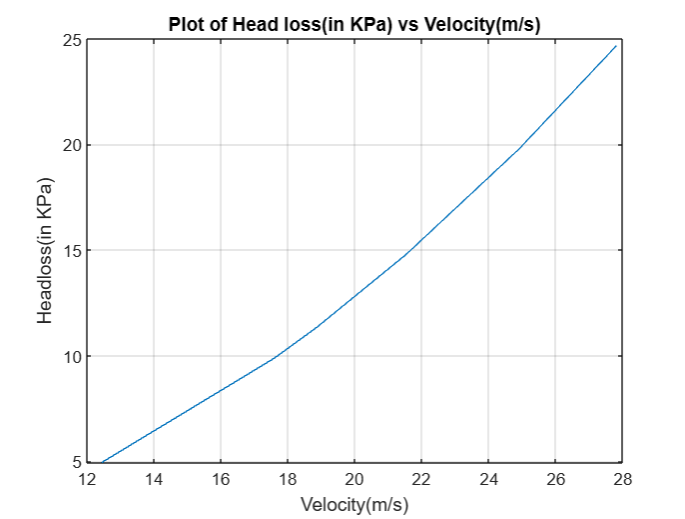
\includegraphics[scale=0.6]{ls 2 img 2.png}
		}
	\end{center}
	\caption{Head loss vs Velocity}
\end{figure}
\newpage
\section{Calculations :}
Calculations are shown for data 1 :
We know,
\begin{equation}
   \alpha = \frac{A_4}{A_1} = \frac{d_4^{2}}{d_1^{2}} = \frac{12^{2}}{34^{2}} = 0.1246
\end{equation}
Due to sudden expansion, head loss per unit volume :
\begin{equation}
    v_1 = \sqrt{\frac{2P_1}{\rho}} = \sqrt{\frac{2\times 400}{1.293}} = 24.90 m/s
\end{equation}
\begin{equation}
    v_4 = \frac{A_1 v_1}{A_4} = \frac{d_1^{2}v_1}{d_4^{2}} = \frac{34^{2} \times 24.90}{12^{2}} = 199.892 m/s
\end{equation}
Head loss per unit volume($H_L$)(Due to sudden expansion) = \begin{equation}
\frac{\rho v_4^{2} (1-\alpha)^{2}}{2}
\end{equation}
\begin{equation}
= \frac{1}{2} \times 1.293 \times 199.892^{2}\times (1-0.1246)^{2}  
\end{equation}
\begin{equation}
= \frac{1}{2} \times 1.293 \times 199.892^{2}\times (1-0.1246)^{2} = 19777.69 Pa\\
\end{equation}
For boundary layer ,head loss per unit volume :
\begin{equation}
    H_b = P_3 - P_4 = -9.9-(-11.1) = 1.2 KPa = 1200 Pa\\
\end{equation}
    Therefore Total loss = $(19.78+1.2)$ Kpa = 20.98 KPa\\
 Percentage loss = $\frac{Headloss due to expansion}{Total loss} \times 100 = 94.28\%$

\section{Sources of Error:}
\begin{itemize}
    \item Error in Manometer.
    \item Error in taking readings due to frequent changes in reading
    \item Error due to environmental effect like temperature,pressure change.
\end{itemize}



\section{Conclusion :}
\begin{itemize}
    \item From calculation of Headloss due to sudden expansion,Boudary Layer Headloss(due to viscous force) and total Headloss we have observed that Headloss due to sudden expansion is the most of the Total Headloss.
    \item There is a pressure drop across the length of pipe due to sudden expansion which is called Dead air Pressure.
    \item From observed data and graphical representation we have observed as velociy of flow increases Headloss also increases.
    \item From data we observed that pressure decreases gradually then increases a little across the length of pipe.
    \item Pressure before expansion is almost same as pressure after expansion.
\end{itemize}

\end{document}